\documentclass[12pt, a4paper, oneside, openright, titlepage]{book}
\usepackage[utf8]{inputenc}
\raggedbottom
\usepackage{import}


%%%%%%%%%%%%%%%%% Book Formatting Comments:

%%%%%%%%%%%%%%%%%%%%%%%%%%%%%%%%%%%%% for Part

%%%%%%%%%%%%%%%%%%%%%% for chapter

%%%%%%%%%%%%%%%%%%%% for section




%%%%%% PACKAGES %%%%%%%
\usepackage{hyperref}
\hypersetup{
    colorlinks,
    citecolor=black,
    filecolor=black,
    linkcolor=black,
    urlcolor=black
}
\usepackage{amsmath} % Math display options
\usepackage{amssymb} % Math symbols
%\usepackage{amsfonts} % Math fonts
%\usepackage{amsthm}
\usepackage{mathtools} % General math tools
\usepackage{array} % Allows you to write arrays
\usepackage{empheq} % For boxing equations
% \usepackage{mathabx}
% \usepackage{mathrsfs}
\usepackage{nameref}
\usepackage{wrapfig}

\usepackage{soul}
\usepackage[normalem]{ulem}

\usepackage{txfonts}
\usepackage{cancel}
\usepackage[toc, page]{appendix}
\usepackage{titletoc,tocloft}
\setlength{\cftchapindent}{1em}
\setlength{\cftsecindent}{2em}
\setlength{\cftsubsecindent}{3em}
%\setlength{\cftsubsubsecindent}{4em}
\usepackage{titlesec}

%\titleformat{\section}
%  {\normalfont\fontsize{25}{15}\bfseries}{\thesection}%{1em}{}
%\titleformat{\section}
%  {\normalfont\fontsize{20}{15}\bfseries}%{\thesubsection}{1em}{}
%\setcounter{secnumdepth}{1}  
  
  

%\newcommand\numberthis{\refstepcounter{equation}\tag{\theequation}} % For equation labelling
\usepackage[framemethod=tikz]{mdframed}

\usepackage{tikz} % For drawing commutative diagrams
\usetikzlibrary{cd}
\usetikzlibrary{calc}
\tikzset{every picture/.style={line width=0.75pt}} %set default line width to 0.75p

\usepackage{datetime}
\usepackage[margin=1.5in]{geometry}
\setlength{\parskip}{1em}
\usepackage{makeidx}         % allows index generation
\usepackage{graphicx}       % standard LaTeX graphics tool
\usepackage{multicol}        % used for the two-column index
\usepackage[bottom]{footmisc}% places footnotes at page bottom

\usepackage{newtxtext}       % 
\usepackage{newtxmath}       % selects Times Roman as basic font
\usepackage{float}
\usepackage{fancyhdr}
\setlength{\headheight}{15pt} 
\pagestyle{fancy}
\lhead[\leftmark]{}
\rhead[]{\leftmark}

%\usepackage{enumitem}

\usepackage{url}
\allowdisplaybreaks

%%%%%% ENVIRONMENTS %%%
\definecolor{purp}{rgb}{0.29, 0, 0.51}
\definecolor{bloo}{rgb}{0, 0.13, 0.80}



%%\newtheoremstyle{note}% hnamei
%{3pt}% hSpace above
%{3pt}% hSpace belowi
%{}% hBody fonti
%{}% hIndent amounti
%{\itshape}% hTheorem head fonti
%{:}% hPunctuation after theorem headi
%{.5em}% hSpace after theorem headi
%{}% hTheorem head spec (can be left empty, meaning ‘normal’)i





% %%%%%%%%%%%%% THEOREM DEFINITIONS

\spnewtheorem{axiom}{Axiom}[chapter]{\bfseries}{\itshape}


\spnewtheorem{construction}{Construction}[chapter]{\bfseries}{\itshape}

\spnewtheorem{props}{Properties}[chapter]{\bfseries}{\itshape}


\renewcommand{\qedsymbol}{$\blacksquare$}


\numberwithin{equation}{section}

\newenvironment{qest}{
    \begin{center}
        \em
    }
    {
    \end{center}
    }

%%%%%% MACROS %%%%%%%%%
%% New Commands
\newcommand{\ip}[1]{\langle#1\rangle} %%% Inner product
\newcommand{\abs}[1]{\lvert#1\rvert} %%% Modulus
\newcommand\diag{\operatorname{diag}} %%% diag matrix
\newcommand\tr{\mbox{tr}\.} %%% trace
\newcommand\C{\mathbb C} %%% Complex numbers
\newcommand\R{\mathbb R} %%% Real numbers
\newcommand\Z{\mathbb Z} %%% Integers
\newcommand\Q{\mathbb Q} %%% Rationals
\newcommand\N{\mathbb N} %%% Naturals
\newcommand\F{\mathbb F} %%% An arbitrary field
\newcommand\ste{\operatorname{St}} %%% Steinberg Representation
\newcommand\GL{\mathbf{GL}} %%% General Linear group
\newcommand\SL{\mathbf{SL}} %%% Special linear group
\newcommand\gl{\mathfrak{gl}} %%% General linear algebra
\newcommand\G{\mathbf{G}} %%% connected reductive group
\newcommand\g{\mathfrak{g}} %%% Lie algebra of G
\newcommand\Hbf{\mathbf{H}} %%% Theta fixed points of G
\newcommand\X{\mathbf{X}} %%% Symmetric space X
\newcommand{\catname}[1]{\normalfont\textbf{#1}}
\newcommand{\Set}{\catname{Set}} %%% Category set
\newcommand{\Grp}{\catname{Grp}} %%% Category group
\newcommand{\Rmod}{\catname{R-Mod}} %%% Category r-modules
\newcommand{\Mon}{\catname{Mon}} %%% Category monoid
\newcommand{\Ring}{\catname{Ring}} %%% Category ring
\newcommand{\Topp}{\catname{Top}} %%% Category Topological spaces
\newcommand{\Vect}{\catname{Vect}_{k}} %%% category vector spaces'
\newcommand\Hom{\mathbf{Hom}} %%% Arrows

\newcommand{\map}[2]{\begin{array}{c} #1 \\ #2 \end{array}}

\newcommand{\Emph}[1]{\textbf{\ul{\emph{#1}}}}




%% Math operators
\DeclareMathOperator{\ran}{Im} %%% image
\DeclareMathOperator{\aut}{Aut} %%% Automorphisms
\DeclareMathOperator{\spn}{span} %%% span
\DeclareMathOperator{\ann}{Ann} %%% annihilator
\DeclareMathOperator{\rank}{rank} %%% Rank
\DeclareMathOperator{\ch}{char} %%% characteristic
\DeclareMathOperator{\ev}{\bf{ev}} %%% evaluation
\DeclareMathOperator{\sgn}{sign} %%% sign
\DeclareMathOperator{\id}{Id} %%% identity
\DeclareMathOperator{\supp}{Supp} %%% support
\DeclareMathOperator{\inn}{Inn} %%% Inner aut
\DeclareMathOperator{\en}{End} %%% Endomorphisms
\DeclareMathOperator{\sym}{Sym} %%% Group of symmetries


%% Diagram Environments
\iffalse
\begin{center}
    \begin{tikzpicture}[baseline= (a).base]
        \node[scale=1] (a) at (0,0){
          \begin{tikzcd}
           
          \end{tikzcd}
        };
    \end{tikzpicture}
\end{center}
\fi




\newdateformat{monthdayyeardate}{%
    \monthname[\THEMONTH]~\THEDAY, \THEYEAR}
%%%%%%%%%%%%%%%%%%%%%%%

%%% Specific Macros %%%


%%%%%% BEGIN %%%%%%%%%%


\begin{document}

%%%%%% TITLE PAGE %%%%%%

\begin{titlepage}
    \centering
    \scshape
    \vspace*{\baselineskip}
    \rule{\textwidth}{1.6pt}\vspace*{-\baselineskip}\vspace*{2pt}
    \rule{\textwidth}{0.4pt}
    
    \vspace{0.75\baselineskip}
    
    {\LARGE Complex Analysis: A Complete Guide}
    
    \vspace{0.75\baselineskip}
    
    \rule{\textwidth}{0.4pt}\vspace*{-\baselineskip}\vspace{3.2pt}
    \rule{\textwidth}{1.6pt}
    
    \vspace{2\baselineskip}
    Complex Analysis \\
    \vspace*{3\baselineskip}
    \monthdayyeardate\today \\
    \vspace*{5.0\baselineskip}
    
    {\scshape\Large Elijah Thompson, \\ Physics and Math Honors\\}
    
    \vspace{1.0\baselineskip}
    \textit{Solo Pursuit of Learning}
    \vfill
    \enlargethispage{1in}
    \begin{figure}[b!]
    \makebox[\textwidth]{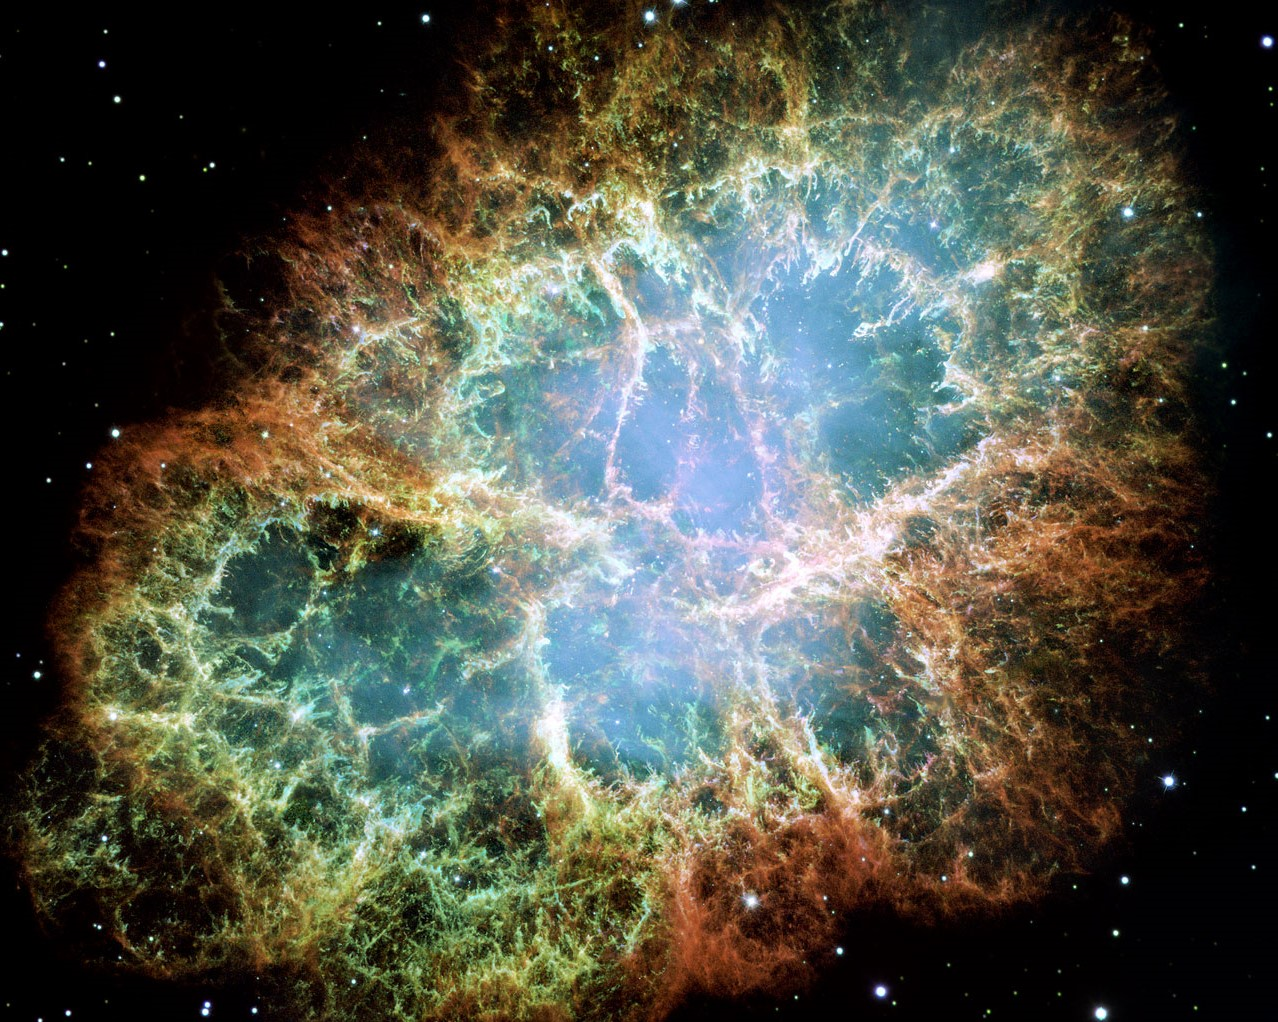
\includegraphics[width=\paperwidth, height =10cm]{../../Crab.jpg}}
    \end{figure}
\end{titlepage}

%%%%%%%%%%%%%%%%%%%%%%%
\tableofcontents


%%%%%%%%%%%%%%%%%%%%%%%%%%%%%%%%%%%%% Part 1.
\part{Part 1}

%%%%%%%%%%%%%%%%%%%%%% Chapter 1.1
\chapter{The Complex Plain and Basic Functions}




%%%%%%%%%%%%%%%%%%%% Section 1.1.1
\section{Complex Numbers}

The complex numbers, $\C$, consist of all formul sums $z = x+iy$, for $x,y \in \R$, where $i^2 = -1$ is the root of $x^2 + 1 = 0$. Then, for multiplication we proceed by $z\cdot w = (a+ib)(x+iy) = (ax-by)+i(xb+ay)$.

Gauss concieved of $\C$ as $\R^2$ with a binary operation $*$, where $(a,b)*(x,y) = (ax-by,xb+ay)$. Then, we observe that $(1,0)*(a,b) = (a,b)$, so $(1,0)$ acts as $1$. Moreover, $(0,1)*(0,1) = (-1,0) = -(1,0)$. 


The matrix model of $\C$ is $$\C = \left\{\begin{bmatrix} a & -b // b & a \end{bmatrix}: a,b \in \R\right\}$$

In terms of extension fields, we can consider $\C$ to be $\R[x]/(x^2+1)$. 

\begin{defn}
    If $z = x+iy$, with $x,y \in \R$, then we define $\mathscr{R}e(z) = x$ and $\mathscr{I}m(z) = y$.
\end{defn}


\begin{defn}
    If $z = x+iy$, we define the \Emph{conjugate} of $z$ to be $\overline{z} x-iy$.
\end{defn}

\begin{props}
    Let $z,w \in \C$. \begin{itemize}
        \item $\overline{z+w} = \overline{z}+\overline{w}$
        \item $\overline{zw} = \overline{z}\cdot \overline{w}$
        \item $\overline{\overline{z}} = z$
        \item $\overline{z} = 0$ if and only if $z = 0$
        \item $\mathscr{R}e(z) = \frac{z+\overline{z}}{2}$
        \item $\mathscr{I}m(z) = \frac{z-\overline{z}}{2i} = \frac{i(\overline{z}-z)}{2}$
    \end{itemize}
\end{props}

\begin{prop}
    If $z \neq 0$, then $z^{-1} = \frac{\overline{z}}{z\overline{z}}$.
\end{prop}


\begin{defn}
    Let $z \in \C$. Then the \Emph{modulus}, $|\cdot |$ of $z=a+ib$ (the norm), is the length of $z$ as a vector: \begin{equation*}
        |z| = \sqrt{a^2+b^2} = \sqrt{z\overline{z}}
    \end{equation*}
\end{defn}


\subsection{Geometry of the Complex Numbers}

The complex numbers, $\C = \{a+ib:a,b \in \R\}$, can be considered as a plane of points, or we can consider the complex numbers as vectors in the plane eminating from $0$. 
\begin{center}
	\begin{tikzpicture}[x=0.75pt,y=0.75pt,yscale=-1,xscale=1]
%uncomment if require: \path (0,398); %set diagram left start at 0, and has height of 398

%Straight Lines [id:da39464285181286485] 
\draw [color={rgb, 255:red, 255; green, 0; blue, 0 }  ,draw opacity=1 ]   (200,310) -- (287.66,212.27) ;
\draw [shift={(289,210.78)}, rotate = 491.89] [color={rgb, 255:red, 255; green, 0; blue, 0 }  ,draw opacity=1 ][line width=0.75]    (10.93,-3.29) .. controls (6.95,-1.4) and (3.31,-0.3) .. (0,0) .. controls (3.31,0.3) and (6.95,1.4) .. (10.93,3.29)   ;
%Straight Lines [id:da13724064512600265] 
\draw  [dash pattern={on 0.84pt off 2.51pt}]  (289,210.78) -- (289.67,309.44) ;
%Shape: Arc [id:dp896874676115538] 
\draw  [draw opacity=0][fill={rgb, 255:red, 74; green, 144; blue, 226 }  ,fill opacity=1 ][dash pattern={on 0.84pt off 2.51pt}] (211.58,297.56) .. controls (212.75,299.62) and (213.81,301.84) .. (214.75,304.19) .. controls (215.48,306.03) and (216.1,307.86) .. (216.61,309.67) -- (199.73,310.18) -- cycle ; \draw  [dash pattern={on 0.84pt off 2.51pt}] (211.58,297.56) .. controls (212.75,299.62) and (213.81,301.84) .. (214.75,304.19) .. controls (215.48,306.03) and (216.1,307.86) .. (216.61,309.67) ;
%Shape: Axis 2D [id:dp8729881414013165] 
\draw  (182.33,310.18) -- (356.33,310.18)(199.73,166.78) -- (199.73,326.11) (349.33,305.18) -- (356.33,310.18) -- (349.33,315.18) (194.73,173.78) -- (199.73,166.78) -- (204.73,173.78)  ;
%Straight Lines [id:da5981962432151724] 
\draw [color={rgb, 255:red, 74; green, 144; blue, 226 }  ,draw opacity=1 ]   (199.73,310.18) -- (130.17,214.18) ;
\draw [shift={(129,212.56)}, rotate = 414.07] [color={rgb, 255:red, 74; green, 144; blue, 226 }  ,draw opacity=1 ][line width=0.75]    (10.93,-3.29) .. controls (6.95,-1.4) and (3.31,-0.3) .. (0,0) .. controls (3.31,0.3) and (6.95,1.4) .. (10.93,3.29)   ;
%Shape: Arc [id:dp8546612577752639] 
\draw  [draw opacity=0][fill={rgb, 255:red, 243; green, 19; blue, 19 }  ,fill opacity=1 ][dash pattern={on 0.84pt off 2.51pt}] (194.73,303.29) .. controls (196.25,302.4) and (198.06,301.89) .. (200,301.89) .. controls (205.33,301.89) and (209.65,305.75) .. (209.67,310.53) -- (200,310.56) -- cycle ; \draw  [dash pattern={on 0.84pt off 2.51pt}] (194.73,303.29) .. controls (196.25,302.4) and (198.06,301.89) .. (200,301.89) .. controls (205.33,301.89) and (209.65,305.75) .. (209.67,310.53) ;

% Text Node
\draw (354,302.4) node [anchor=north west][inner sep=0.75pt]    {$\mathscr{R} e$};
% Text Node
\draw (184.5,151.07) node [anchor=north west][inner sep=0.75pt]    {$\mathscr{I} m$};
% Text Node
\draw (290,199.51) node [anchor=north west][inner sep=0.75pt]  [font=\scriptsize]  {$z=a+ib$};
% Text Node
\draw (220,312.18) node [anchor=north west][inner sep=0.75pt]  [font=\scriptsize]  {$a=|z|\cos \theta $};
% Text Node
\draw (292.67,254.84) node [anchor=north west][inner sep=0.75pt]  [font=\scriptsize]  {$ib=i|z|\sin \theta $};
% Text Node
\draw (218,294.51) node [anchor=north west][inner sep=0.75pt]  [font=\scriptsize]  {$\theta $};
% Text Node
\draw (202.67,286.62) node [anchor=north west][inner sep=0.75pt]  [font=\scriptsize]  {$\beta $};
% Text Node
\draw (100,200.29) node [anchor=north west][inner sep=0.75pt]  [font=\scriptsize]  {$w=x+iy$};

\draw   (122.72, 166.5) circle [x radius= 5, y radius= 5]   ;
\draw   (123.55, 165.96) circle [x radius= 5, y radius= 5]   ;
\draw   (288.47, 51.73) circle [x radius= 5, y radius= 5]   ;
\draw   (372.18, 109) circle [x radius= 5, y radius= 5]   ;
\draw   (537.1, 23.04) circle [x radius= 5, y radius= 5]   ;
\draw   (249.38, 297.62) circle [x radius= 5, y radius= 5]   ;
\draw   (376.5, 243.59) circle [x radius= 5, y radius= 5]   ;
\draw   (414.3, 248.15) circle [x radius= 5, y radius= 5]   ;
\end{tikzpicture}	
\end{center}


Noting this geometric picture, we can write $z = |z|\cos\theta+i|z|\sin\theta = |z|(\cos\theta + i\sin\theta)$. Suppose we had another complex number $w = |w|(\cos\beta+i\sin\beta)$. Then we observe that \begin{align*}
    zw &= |z||w|(\cos\theta+i\sin\theta)(\cos\beta+i\sin\beta) \\
    &= |zw|(\cos\theta\cos\beta -\sin\theta\sin\beta + i(\sin\theta\cos\beta+\cos\theta\sin\beta)) \\
    &= |zw|(\cos(\theta+\beta)+i\sin(\theta+\beta))
\end{align*}
so complex multiplication aligns with angle addition in the plane.


\begin{defn}
    Define \Emph{Euler's Formula} \begin{equation*}
        e^{i\theta} = \cos\theta+i\sin\theta
    \end{equation*}
\end{defn}

From our above work we have that \begin{equation*}
    zw = (|z|e^{i\theta})(|w|e^{i\beta}) = |zw|e^{i(\theta+\beta)}
\end{equation*}
so \begin{equation*}
    e^{i\theta}e^{i\beta} = e^{i(\theta+\beta)}
\end{equation*}
The conjugate of $e^{i\theta}$ is \begin{equation*}
    \overline{e^{i\theta}} = \overline{\cos\theta+i\sin\theta} = \cos\theta-i\sin\theta=\cos(-\theta)+i\sin(-\theta) = e^{-i\theta}
\end{equation*}


\begin{prop}
    $e^{i\theta} = e^{i\beta}$ if and only if $\theta = \beta + 2\pi k$ for some $k \in \Z$.
\end{prop}

Then we have that $e^{i\theta} = e^{-i\theta}$ if and only if $\theta = \pi k$ for some $k \in \Z$.

\begin{defn}
    Let $z \in \C$. The \Emph{argument} of $z = |z|e^{i\theta}$ is $\arg(z) = \{\theta+2\pi k:k \in \Z\}$, and the \Emph{principal argument} of $z$, $\text{Arg}(z) = \theta_0$, where $z = |z|e^{i\theta_0}$ and $\theta_0 \in (-\pi,\pi]$.
\end{defn}


\begin{eg}
    Consider $z = -42-42i$. Then $|z| = 42\sqrt{2}$, and $\text{Arg}(z) = -\frac{3\pi}{4}$, so $z = 42\sqrt{2}e^{-i\frac{3\pi}{4}}$, and $\arg(z) = -\frac{3\pi}{4} + 2\pi\Z$.
\end{eg}

\begin{props}
    For $z,w \in \C$, $\arg(zw) = \arg(z)+\arg(w)$, but $\text{Arg}(zw) \neq \text{Arg}(z)+\text{Arg}(w)$.
\end{props}

\begin{thm}[DeMoivre's Theorem] \label{thm:DeMoivre}
    For all $n \in \Z$, \begin{equation*}
        (e^{i\theta})^n = e^{in\theta}
    \end{equation*}
\end{thm}
\begin{proof}
    We proceed by induction on $n \in \N$. If $n=1$ then $(e^{i\theta})^1 = e^{i1\theta}$, so the base case holds. Now, suppose that the claim holds for some $n \geq 1$. It follows that \begin{align*}
        (e^{i\theta})^{n+1} &= (e^{i\theta})^1(e^{i\theta})^n \\ 
        &= e^{i\theta}e^{in\theta} \tag{by I.H} \\
        &= e^{i(\theta+n\theta)} \\
        &= e^{i(n+1)\theta}
    \end{align*}
    completing the proof.
\end{proof}



\begin{defn}
    Suppose that $n \in \N$, $w,z \in \C$ such that $z^n = w$, then $z$ is said to be an \Emph{$n$th root of $w$}. Moreover, the set of all $n$th roots is dentoed $w^{1/n} \neq \sqrt[n]{w}$.
\end{defn}

Let $z^n = w$, where $z = \rho e^{i\theta}$. Then it follows that \begin{align*}
    (\rho e^{i\theta})^n &= w \\
    \rho^ne^{in\theta} &= |w|e^{i\text{Arg}(w)} \tag{by \ref{thm:DeMoivre}}
\end{align*}
This gives the two equations $\rho^n = |w|$ and $e^{in\theta} = e^{i\text{Arg}(w)}$, so $\rho = \sqrt[n]{|w|}$, and \begin{align*}
    n\theta &= \text{Arg}(w)+2\pi k \\
    \theta &= \frac{\text{Arg}(w)}{n}+\frac{2\pi k}{n}
\end{align*}
This gives the following result: 
\begin{cor}
    $$w^{1/n} = \left\{\sqrt[n]{|w|}e^{i\frac{\text{Arg}(w)}{n}}e^{i\frac{2\pi k}{n}}: k \in \Z\right\}$$
\end{cor}
\begin{defn}
    If $w = 1$, we have that \begin{equation*}
        1^{1/n} = \left\{e^{i\frac{2\pi k}{n}}:k\in \Z\right\}
    \end{equation*}
    These are the \Emph{$n$th roots of unity}.
\end{defn}

Then we observe that for any $w \in \C$, $$w^{1/n} = \sqrt[n]{|w|}e^{i\frac{\text{Arg}(w)}{n}}1^{1/n}$$


\begin{eg}
    Consider the fourth roots of $81i$, so $(81i)^{1/4}$. Then we have that \begin{align*}
        (81i)^{1/4} &= \sqrt[4]{81}e^{i\frac{\pi}{8}}1^{1/4} \\
        &= 3e^{i\frac{\pi}{8}}\{1,i,-1,-i\}
    \end{align*}
\end{eg}

\begin{eg}
    Let $w = \exp\left(\frac{2\pi i}{6}\right)$. Then \begin{align*}
        1^{1/6} &= \{z \in \C:z^6 = 1\} = \{w,w^2,w^3,w^4,w^5,w^6 = 1\}
    \end{align*}
    Note $w = e^{i\pi/3} = \cos(\pi/3)+i\sin(\pi/3) = \frac{1+i\sqrt{3}}{2}$. Now, if we consider the polynomial $f(z) = z^6 - 1$, we now know six roots for this polynomial. Then we can factor \begin{equation*}
        f(z) = \prod_{i=1}^6(z-w^i)
    \end{equation*}
    In short, to solve $z^n = \rho$, we take the $n$th roots of $\rho$, $\rho^{1/n}$. 
\end{eg}



\begin{eg}
    Consider $z^2+bz+c = 0$. Then completing the square we obtain $z \in \left\{\frac{-b+ (b^2-4c)^{1/2}}{2}\right\}$, where \begin{equation*}
        \left(\frac{b^2-4c}{2}\right)^{1/2} = \left\{\begin{array}{ccc} \sqrt{\left|\frac{b^2-4c}{2}\right|} & -\sqrt{\left|\frac{b^2-4c}{2}\right|} & if\;b^2-4c \geq 0 \\ \sqrt{\left|\frac{b^2-4c}{2}\right|}i & -\sqrt{\left|\frac{b^2-4c}{2}\right|}i & if\; b^2-4c < 0 \end{array}\right\}
    \end{equation*}
\end{eg}


%%%%%%%%%%%%%%%%%%%% Section 1.1.2
\section{Local Inverses and Branch-cut}

\begin{defn}    
    Let $z,w \in \C$, then the line segment from $z$ to $w$ is \begin{equation*}
        [z,w] = \{z+t(w-z):0\leq t \leq 1\}
    \end{equation*}
    where we also allow $z$ or $w$ to be plus or minus infinity.
\end{defn}

\begin{defn}
    The \Emph{negative slit plane}, $\C^-$, is defined by $\C^- = \C\backslash(-\infty,0]$, and the \Emph{positive slit plane}, $\C^+$, is defined by $\C^+ = \C\backslash[0,\infty)$. In general, we define \begin{equation*}
        C^{\alpha} = \C\backslash[0,e^{i\alpha}\infty)
    \end{equation*}
    to denote the exclusion of the ray along the $\alpha$th angle from the positive real axis.
\end{defn}

\begin{qst}
    What is a function?
\end{qst}

\begin{defn}
    If $f:S\rightarrow \C$ is a function, and $U \subseteq S$, then $f\vert_U:U\rightarrow \C$ is defined by $f\vert_U(z) = f(z)$ for all $z \in U$.
\end{defn}

We may have the case that $f$ is not injective (so it cannot be inverted). But, for a smart choice of $U$, we may have that $f\vert_U$ is one-to-one, and hence invertible. Such a restriction is known as a \Emph{local inverse} for $f$.

Rigourously, a \Emph{branch cut} is a curve in the complex plane such that it is possible to define a single analytic branch (sheets of a multivalued function) of a multivalued function on the plane minus that curve. That is, a branch is a way of making the multivalued function single valued, and in the context of determining inverses a branch is a choice of inverse.

\begin{eg}
    For $f(z) = z^n$, then for $U = \left\{z \in \C: -\frac{\pi}{n}<\text{Arg}(z) < \frac{\pi}{n}\right\}$, $f\vert_{U}$ is invertible, and $f\vert_{U}^{-1}$ is called the \Emph{principal branch}. $f\vert_U^{-1}$ is a choice of the $n$th root of $w \in \C^-$. 
\end{eg}


\begin{defn}
    The \Emph{$\alpha$-argument} for $\alpha \in \R$ is denoted $\text{Arg}_{\alpha}:\C^{\times}\rightarrow (\alpha,\alpha+2\pi)$. In particular, for each $z \in \C^{\times}$ we define $\text{Arg}_{\alpha} \in \arg(z)$ such that $z \in (\alpha,\alpha+2\pi)$
\end{defn}

We can give branch cuts for the $n$th root function which delete the ray at standard angle $\alpha$. These correspond to local inverse functions $f(z) = z^n$ restricted to $\{z \in \C^{\times}:\arg(z) = (\alpha/n,(\alpha+2\pi)/2)+2\pi\Z\}$.


\subsection{Square-Root Function}

If we have $z^2 = w$, this is equivalent to $(|z|e^{i\theta})^2 = |w|e^{i\beta}$, so $|z|^2=|w|$ and $e^{i2\theta} = e^{i\beta}$. Then $|z| = \sqrt{|w|}$, and $\theta = \frac{\beta}{2} + \pi k$ for $k \in \Z$. Then our solutions are \begin{equation*}
    z = \sqrt{|w|}e^{i(\beta/2+\pi k)} = \sqrt{|w|}e^{i\beta/2}e^{i\pi k} = \sqrt{|w|}e^{i\beta/2}\cos(\pi k)
\end{equation*}
Thus, in general \begin{equation*}
    z = \sqrt{|w|}e^{i\text{Arg}(w)/2}(-1)^k = \pm \sqrt{|w|}e^{i\text{Arg}(w)/2}
\end{equation*}
and \begin{equation*}
    w^{1/2} = \{\sqrt{|w|}e^{i\text{Arg}(w)/2}, -\sqrt{|w|}e^{i\text{Arg}(w)/2}\}
\end{equation*}
In general we have \begin{equation*}
    w^{1/n} = \{\sqrt[n]{w},\zeta\sqrt[n]{w},...,\zeta^{n-1}\sqrt[n]{w}\}
\end{equation*}
where $\sqrt[n]{w} = \sqrt[n]{|w|}\exp\left(\frac{i\text{Arg}(w)}{n}\right)$ is the principal root, and $\zeta = e^{\frac{2\pi i}{n}}$ is an $n$th root of unity. The principal root is the local inverse for the principal branch $U = 
\{z:-\pi/n < \text{Arg}(z) < \pi/n\}$. 


%%%%%%%%%%%%%%%%%%%% Section 1.1.3
\section{Complex Exponential}

\begin{defn}
    We define the complex exponential for $z \in \C$ to be \begin{equation*}
        e^z = e^{\mathscr{R}e(z)}e^{i\mathscr{I}m(z)} = e^{\mathscr{R}e(z)}(\cos(\mathscr{I}m(z))+i\sin(\mathscr{I}m(z)))
    \end{equation*}
\end{defn}

\begin{props}
    Let $z = x+iy, w = a+ib \in \C$. \begin{itemize}
        \item $e^ze^w = e^{z+w}$
        \item $|e^{x+iy}| = |e^x||e^{iy}| = e^x$, which is never zero so the complex exponential is never zero. that is,
        \item $e^z \neq 0$ for all $z \in \C$.
        \item $\arg(e^z) = \arg(e^xe^{iy}) = y+2\pi\Z$.
    \end{itemize}
\end{props}


\subsection{Failure to Inject}

If $e^{z_1} = e^{z_2}$, then $e^{x_1}e^{iy_1} = e^{x_2}e^{iy_2}$, so $x_1 = x_2$ and $y_1 \in y_2 + 2\pi\Z$. Thus, $e^z$ has a $2\pi i$-periodicity; $e^z = e^{z+2\pi ik}$ for $k \in \Z$. To make the complex exponential, we must restrict the domain to some horizontal strip of height at most $2\pi$ (with endpoints not included). In particular, if we take $U = \{x+iy: -\pi < y < \pi\}$ we obtain the branch $\C^-$, and branch cut $(-\infty,0]$. Then, suppose we write $e^z = w = |w|e^{i\text{Arg}(w)}$. Then a solution is $e^x = |w|$, and $y = \text{Arg}(w)$. We can then define \begin{equation*}
    \text{Log}(w) = \ln|w| +i\text{Arg}(w) = z = x+iy
\end{equation*}
for $w \in \C^-$, which is the branch cut to the multivalued log \begin{equation*}
    \log(z) = \ln|z|+i\arg(z)
\end{equation*}
taking the restriction $U$ in the range.



%%%%%%%%%%%%%%%%%%%% Section 1.1.4
\section{Sine, Cosine, Cosh, Sinh}

Recall $e^{i\theta} = \cos\theta +i\sin\theta$ and $e^{-i\theta} = \cos\theta-i\sin\theta$. Then we have that \begin{equation*}
    e^{i\theta}+e^{-i\theta}=2\cos\theta
\end{equation*}
and \begin{equation*}
    e^{i\theta}-e^{-i\theta} = 2i\sin\theta
\end{equation*}
Thus, we can obtain formulas for $\sin$ and $\cos$, $\theta \in \C$: \begin{equation*}
    \cos\theta = \frac{e^{i\theta}+e^{-i\theta}}{2}
\end{equation*}
and \begin{equation*}
    \sin\theta = \frac{e^{i\theta}-e^{-i\theta}}{2i}
\end{equation*}
Then we define:

\begin{defn}
    We define the complex sine and cosine, $z \in \C$, by \begin{equation}
        \boxed{\cos z = \frac{e^{iz}+e^{-iz}}{2}}
    \end{equation}
    and \begin{equation}
        \boxed{\sin z = \frac{e^{iz}-e^{-iz}}{2i}}
    \end{equation}
\end{defn}

Observe that \begin{equation*}
    e^x = \underbrace{\frac{1}{2}(e^x+e^{-x})}_{\cosh(x)} + \underbrace{\frac{1}{2}(e^x-e^{-x})}_{\sinh(x)}
\end{equation*}
\begin{defn}
    We define the complex hyperbolic sine and hyperbolic cosine, $z \in \C$, by \begin{equation}
        \boxed{\cosh z = \frac{e^{z}+e^{-z}}{2}}
    \end{equation}
    and \begin{equation}
        \boxed{\sinh z = \frac{e^{z}-e^{-z}}{2}}
    \end{equation}
\end{defn}

Then we have the identities \begin{equation*}
    \cosh z = \cos(iz), \sinh z = -i\sin(iz)
\end{equation*}
and \begin{equation*}
    \cos(z) = \cosh(iz), \sin z = -i\sinh(iz)
\end{equation*}

\subsection{Complex Cosine is Not Bounded}

Observe \begin{equation*}
    \cos(z) = \cos(x+iy) = \frac{e^{ix-y}+e^{-ix+y}}{2} = \frac{e^{ix}e^{-y}+e^{-ix}e^y}{2}
\end{equation*}
Now, using angle formulas we have \begin{align*}
    \cos(z) &= \cos(x+iy) \\
    &= \cos(x)\cos(iy)-\sin(x)\sin(iy) \\
    &= \cos(x)\cosh(y)-i\sin(x)\sinh(y)
\end{align*}
so \begin{equation*}
    |\cos z|^2 = \cos^2x\cosh^2y+\sin^2x\sinh^2y = \cos^2x+\sinh^2y
\end{equation*}
so as $\cosh$ and $\sinh$ are unbounded, so is complex $\cos$. 

\begin{claim}
    \begin{align*}
        \cos(z+w) &= \cos(z)\cos(w)-\sin(z)\sin(w) \\
        \sin(z+w) &= \sin(z)\cos(w)+\sin(w)\cos(z) 
    \end{align*}
    and \begin{align*}
        \cosh(z+w) &= \sinh z\sinh w + \cosh z\cosh w \\
        \sinh(z+w) &= \sinh z\cosh w + \cosh z\sinh w
    \end{align*}
\end{claim}


\begin{claim}
    $\cos^2z+\sin^2z = 1$
\end{claim}
\begin{proof}
    First, observe \begin{equation*}
        \cos^2z = \left[\frac{1}{2}(e^{iz}+e^{-iz})\right]^2 = \frac{1}{4}(e^{2iz}+2+e^{-2iz})
    \end{equation*}
    and \begin{equation*}
        \sin^2z = \left[\frac{1}{2i}(e^{iz}-e^{-iz})\right]^2 = \frac{-1}{4}(e^{2iz}-2+e^{-2iz})
    \end{equation*}
    Hence, indeed, $\cos^2z + \sin^2z = 1$.
\end{proof}


%%%%%%%%%%%%%%%%%%%% Section 1.1.5
\section{Power Functions}

\begin{defn}
    Let $\alpha \in \C$ be arbitrary. For $z \in \C^{\times}$ we define the power function $z^{\alpha}$ to be the multivalued function \begin{equation*}
        z^{\alpha} = e^{\alpha\log z}
    \end{equation*}
    Thus, the values of $z^{\alpha}$ are given by \begin{align*}
        z^{\alpha} &= e^{\alpha(\log|z| +i\arg(z))} \\
        &= e^{\alpha\text{Log}(z)}e^{2\pi i\alpha m}, m = 0, \pm 1,\pm 2,...
    \end{align*}
\end{defn}

Consequently, the various values of $z^{\alpha}$ are obtained by multiplying the principal value $e^{\alpha\text{Log}|z|}$ by the integer power of $e^{2\pi i\alpha}$. Consequently, if $\alpha$ is itself an integer $e^{2\pi i\alpha} = 1$, and the power function is single valued and equal to the principal value, $e^{\alpha\text{Log}|z|}$. If $\alpha = 1/n$, for $n \in \N$, then the factor is precisely the $n$th roots of unity, and $z^{1/n}$ are the $n$th roots of unity of $z$.

It is important to note that the usual algebraic rules do not apply to power functions when they are multivalued. 

To haze the power function move continuously with $z$ we make the branch cut $[0,\infty)$. Then we define a continuous branch on $\C^+$ to be \begin{equation*}
    w = r^{\alpha}e^{i\alpha \theta},\; \text{ for }\;z = re^{i\theta}, 0<\theta < 2\pi
\end{equation*}
At the top edge of the slit, $\theta = 0$, we have the usual power function $r^{\alpha} = e^{\alpha\text{Log}r}$. At the bottom of the slit, $\theta = 2\pi$, we have the function $r^{\alpha}e^{2\pi i\alpha}$. For a fixed $r$, as $\theta$ ranges the values of $w= r^{\alpha}e^{i\theta\alpha}$ move continuously. Thus, the values of this branch of $z^{\alpha}$ on the bottom edge are $e^{2\pi i\alpha}$ times the values at the top edge. This multiple, $e^{2\pi i\alpha}$, is called the \Emph{phase factor} of $z^{\alpha}$ at $z = 0$. 

For any other choice of branch, $w=r^{\alpha}e^{i\alpha(\theta+2\pi m)}$, the same phase factor is observed. 

\begin{lem}[Phase Change Lemma]\label{lem:phasechange}
    Let $g(z)$ be a single-valued function that is defined and continuous near $z_0$. For any continuously varying branch of $(z-z_0)^{\alpha}$ the function $f(z) = (z-z_0)^{\alpha}g(z)$ is multiplied by the phase factor $e^{2\pi i \alpha}$ when $z$ traverses a complete circle about $z_0$ in the positive direction.
\end{lem}




%%%%%%%%%%%%%%%%%%%%%% Chapter 1.2
\chapter{Analytic Functions}

%%%%%%%%%%%%%%%%%%%% Section 1.2.1
\section{Basic Analysis and Topology}


\begin{defn}
    A \Emph{sequence} of complex numbers is a function $f:\N\rightarrow \C$, where $f(i) = a_i$ for each $i \in \N$. We often write this sequence as $\{a_n\}_{n=1}^{\infty}$.
\end{defn}

\begin{defn}
    We say a sequence $\{a_n\}_{n=1}^{\infty}$ converges to a limit $L \in \C$, $a_n\rightarrow L$, as $n$ approaches infinity, $n\rightarrow \infty$, if for each $\varepsilon > 0$, there exists $N \in \N$ such that for $n \geq N$, $|a_n - L| < \varepsilon$. We also write \begin{equation*}
        \lim\limits_{n\rightarrow \infty}a_n = L
    \end{equation*}
\end{defn}

That is, if we pick a particular limiting value for the limit value, we can find a point past which the tail of the sequence is between limiting value and our limit.

\begin{defn}
    A sequence $\{a_n\}_{n=1}^{\infty} \subseteq \C$ is said to be \Emph{bounded} if there exists $M \in \R$ such that for all $n \in \N$, $|a_n| < M$ (where $|\cdot|$ is the modulus).
\end{defn}

That is, all points in the sequence exist in an $M$ radius disk of the origin in the complex plane. 

\begin{eg}
    Consider a sequence $a_n = (e^{ir})^n$, where $r \notin \Q$. Then $|a_n| = 1$, for all $n$. Then $\lim\limits_{n\rightarrow \infty}|a_n| = 1$, but the sequence itself does not cnverge in $\C$.
\end{eg}


\begin{thm}
    Suppose $s_n\rightarrow s$ and $t_n\rightarrow t$ for sequences in $\C$. Then \begin{itemize}
        \item $s_n+t_n\rightarrow s+l$
        \item $cs_n \rightarrow cs$, for all $c \in \C$
        \item $s_nt_n \rightarrow st$
        \item $s_n/t_n\rightarrow s/t$, provided $t \neq 0$.
    \end{itemize}
\end{thm}

We remark that the squeeze theorem only applies for real-sequences, as it relies on the ordering of the reals. Moreover, the theorem that ``A bounded monotone sequence of real numbers converges" also does not hold, again due to ordering.

\begin{defn}
    Let $(a_n)$ be a sequence. Let $n_1 < n_2 < n_3 < ...$ be an increasing sequence of natural numbers. Then $\{a_{n_k}\}_{k=1}^{\infty}$ is a \Emph{subsequence} of the sequence $(a_n)$.
\end{defn}

\begin{eg}
    Consider the sequence $(-1)^n$. Then we have that \begin{equation*}
        \lim\sup\limits_{n\rightarrow\infty}(-1)^n = 1,\;\;\text{ and }\;\;\lim\inf\limits_{n\rightarrow\infty}(-1)^n = -1
    \end{equation*}
\end{eg}


\begin{thm}
    Suppose $z_n = x_n+iy_n$ for real sequences $x_n$ and $y_n$. Let $z = x+iy \in \C$. Then $z_n\rightarrow z$ if and only if $x_n\rightarrow x$ and $y_n\rightarrow y$.
\end{thm}
\begin{proof}
    $\implies$. Assume that $z_n\rightarrow z$. Hence, for each $\varepsilon > 0$, there exists $N \in \N$ such that if $n \geq N$ then $|z_n - z| < \varepsilon$. Consider $|x_n - x|$. Then observe that $|x_n-x| = \sqrt{(x_n-x)^2}\leq \sqrt{(x_n-x)^2+(y_n-y)^2} = |z_n - z$. Then for any $n \geq N$ we have that $|x_n - x| \leq |z_n - z| < \varepsilon$, and similarly, $|y_n - y| \leq |z_n - z| < \varepsilon$. Hence, $x_n\rightarrow x$ and $y_n\rightarrow y$, as desired.

    $\impliedby$. Now, suppose that $x_n\rightarrow x$ and $y_n\rightarrow y$. Fix $\varepsilon > 0$. Then there exist $N_1,N_2 \in \N$ such that $n_1 \geq N_1$ and $n_2 \geq N_2$ imply $|x_{n_1} - x| < \varepsilon/2$ and $|y_{n_2}-y| < \varepsilon$. Let $N = \max(N_1,N_2)$. Then for all $n \geq N$, \begin{equation*}
        |z_n - z| \leq |x_n - x| + |i(y_n - y)| = |x_n - x| + |y_n - y| < \varepsilon/2+\varepsilon/2 = \varepsilon
    \end{equation*}
    Hence, we conclude that $z_n\rightarrow z$, as desired.
\end{proof}

\begin{defn}
    A sequence $\{z_n\}_{n=1}^{\infty}$ is said to be \Emph{Cauchy} if for every $\varepsilon > 0$, there exists $N \in \N$ such that for all $n,m \geq N$, \begin{equation*}
        |z_n - z_m| < \varepsilon
    \end{equation*}
\end{defn}

Thus, the tail of a Cauchy sequence gets arbitrarily close as we go arbitrarily far.

$\C$ is a complete metric space, so the Cauchy sequences are precisely the convergent sequences.


\begin{defn}
    An open disk of radius $\varepsilon > 0$ centered at $z_0 \in \C$ is defined to be \begin{equation*}
        D_{\varepsilon}(z_0) := \{z \in \C: |z-z_0| < \varepsilon\}
    \end{equation*}
\end{defn}

\begin{defn}
    Let $S \subseteq \C$ and $z_0 \in S$. Then $z_0$ is an \Emph{interior point} if there exists $\varepsilon > 0$ such that $D_{\varepsilon}(z_0) \subseteq S$. 

    We say that $S$ is an \Emph{open set} in $\C$ if each point in $S$ is an interior point.
\end{defn}

\begin{defn}
    We say that $S \subseteq \C$ is a \Emph{closed set} if and only if $\C\backslash S$ is open.
\end{defn}

\begin{eg}
    Consider the half-plane $S = \{z \in \C: \mathscr{I}m(z) \geq 1\}$. This is not a closed set as all points on the boundary ($\mathscr{I}m(z) = 1$) are not interior.
\end{eg}

\begin{defn}
    Let $S \subseteq \C$ and $z_0 \in \C$. Then $z_0$ is said to be a \Emph{limit/accumulation point} of $S$ if for every $\varepsilon > 0$, $D_{\varepsilon}^*(z_0)\cap S \neq \emptyset$. 
\end{defn}
That is, neighborhoods of limit points always intersect the set in a point different from the limit point.

\begin{defn}
    Let $f:S\rightarrow \C$ be a complex function, $S \subseteq \C$. Suppose $z_0 \in \C$ is a limit point of $S$. Then we say that $f(z) \rightarrow L$, for $L \in \C$, if and only if for every $\varepsilon > 0$, there exists $\delta > 0$ such that if $0 < |z-z_0| < \delta$, then $|f(z) - L| < \varepsilon$. 


    Equivalently, the functional limit converges to $L$ if and only if for every $\varepsilon > 0$, there exists $\delta > 0$ such that \begin{equation*}
        f(D_{\delta}^*(z_0)\cap S) \subseteq D_{\varepsilon}(L)
    \end{equation*}
\end{defn}


\begin{thm}
    Let $f:S\rightarrow \C$ and $g:U\rightarrow \C$ be complex functions such that $\lim\limits_{z\rightarrow z_0}f(z) = L$ and $\lim\limits_{z\rightarrow z_0}g(z) = M$ for some $L,M \in \C$. Let $c \in \C$. Then\begin{itemize}
        \item $\lim\limits_{z\rightarrow z_0}(f(z)+g(z)) = L+M$
        \item $\lim\limits_{z\rightarrow z_0}cf(z) = cL$
        \item $\lim\limits_{z\rightarrow z_0}f(z)g(z) = LM$
        \item $\lim\limits_{z\rightarrow z_0}f(z)/g(z) = L/M$, provided $M \neq 0$.
    \end{itemize}
\end{thm}

\begin{defn}
    We say that $f:S\rightarrow \C$ is continuous at $z_0 \in S$ if and only if $\lim\limits_{z\rightarrow z_0}f(z) = f(z_0)$.
\end{defn}

\begin{thm}
    Let $f:S\rightarrow \C$. Then $\lim\limits_{z\rightarrow z_0}f(z) = L$ if and only if for all sequences $z_n$ such that $z_n\rightarrow z_0$, $\lim\limits_{n\rightarrow\infty}f(z_n) = L$.
\end{thm}


\begin{defn}
    A subset $S \subseteq \C$ is connected if and only if there exists no $A,B\subseteq \C$ non-empty such that $S = A\cup B$ and $\overline{A}\cap B = \emptyset$ and $A\cap \overline{B} = \emptyset$.
\end{defn}

Noting that connected and path-connected subsets are equivalent in $\C$, we formulate (path) connectedness in another way as follows:

\begin{defn}
    A \Emph{polygonal chain} $P$ is a curve composed of a finite number of connected line segments. That is, there exist $z_0,z_1,...,z_n \in \C$ such that \begin{equation*}
        P = [z_0,z_1] \cup [z_1,z_2] \cup ... \cup [z_{n-1},z_n]
    \end{equation*}
\end{defn}

\begin{defn}
    A subset $U \subseteq \C$ is (path) \Emph{connected} if and only if for each $p,q \in U$, there exists a polygonal chain $\gamma$ which begins at $p$ and terminates at $q$, and $\gamma \subseteq U$.
\end{defn}
    


\begin{defn}
    A subset $D \subseteq \C$ is called a \Emph{domain} if $D$ is both open and connected.
\end{defn}


\begin{defn}
    A \Emph{region} is a domain paired with some or all of its topological boundary.
\end{defn}

\begin{defn}
    Let $U \subseteq \C$. Then $U^o$ denotes the \Emph{interior} of $U$, and is the set of all interior points in $U$.
\end{defn}

\begin{defn}
    A set $U \subseteq \C$ is \Emph{compact} if and only if (Heine-Borel) $U$ is closed and bounded.
\end{defn}


\begin{defn}
    A set $U \subseteq \C$ is said to be \Emph{star-shaped} at a point $z_0 \in \C$ if $z_0 \in U$, and for any $z \in U$ we have $[z_0,z] \subseteq U$.
\end{defn}

Star-shaped implies simply connected: every closed curve in the region can be continuously deformed to a point.

\begin{eg}
    The slit complex plane $\C^- = \C\backslash(-\infty,0]$ is star shaped, with any point along $(0,\infty)$ serving as a star center. In particular, consider the star center $1$. Then, let $z \in \C^-$ and consider $[1,z] = \{1+t(z-1):0\leq t\leq 1\}$. Then, for each $a+ib \in [1,z]$ we have $a+ib = 1+t(x+iy-1) = 1+(x-1)t+iyt$ for some $t \in [0,1]$. For $z \in (0,\infty)$ we have that $y = 0$, and $x-1 > -1$, so $(x-1)t > -1t > -1$, so $a+ib = a > 0$. On the other hand, if $z \in \C^-$ with $y \neq 0$, then $a+ib \notin (-\infty,0]$ for all $t > 0$, and by construction $a+ib = 1$ for $t = 0$, which is again not in $(-\infty,0]$. Thus, $[1,z] \cap (-\infty,0] = \emptyset$ for all $z \in \C^-$, as claimed.
\end{eg}


\begin{thm}\label{thm:constant}
    If $h:D\subseteq \R^2\rightarrow\R^2$ is continuously differentiable on $D$ and $\nabla h= \vec{0}$ on $D$, then $h$ is constant on $D$.
\end{thm}
\begin{proof}
    Let $\gamma:[t_0,t_1]\rightarrow D$ be a polygonal chain in $D$, with $\gamma(t_0) = p$ and $\gamma(t_1) = q$. Then \begin{equation*}
        \frac{d}{dt}(h(\gamma(t)) = \nabla h(\gamma(t)) \cdot \frac{d\gamma}{dt} = 0
    \end{equation*}
    since the gradient is zero in $D$. Then by properties of single variable differentiable functions, $h(\gamma(t))$ is constant so $h(p) = h(\gamma(t_0)) = h(\gamma(t_1)) = h(q)$. But this is true for all $p,q \in D$, so $h$ is constant.
\end{proof}



%%%%%%%%%%%%%%%%%%%% Section 1.2.2
\section{Analytic Functions}

\begin{defn}
    Let $f:S\rightarrow \C$. If the limit \begin{equation*}
        \lim\limits_{z\rightarrow z_0}\left(\frac{f(z) - f(z_0)}{z-z_0}\right)
    \end{equation*}
    exists, we say $f$ is \Emph{complex differentiable} at $z_0$, and we denote \begin{equation*}
        f'(z_0) = \lim\limits_{z\rightarrow z_0}\left(\frac{f(z) - f(z_0)}{z-z_0}\right)
    \end{equation*}
    Futhermore, the mapping $z\mapsto f'(z)$ is the complex derivative of $f$.
\end{defn}

\begin{eg}
    Consider $f(z) = 2z^2 - 1$. Then \begin{equation*}
        \lim\limits_{z\rightarrow z_0}\left(\frac{f(z) - f(z_0)}{z-z_0}\right) = \lim\limits_{z\rightarrow z_0}\left(\frac{2z^2 - 1 - (2z_0^2 - 1)}{z-z_0}\right) = 2\lim\limits_{z\rightarrow z_0}\left(\frac{(z-z_0)(z+z_0)}{z-z_0}\right) = 2\cdot 2z_0 = 4z_0
    \end{equation*}
\end{eg}

\begin{namthm}[Caratheodory Theorem]\label{namthm:car}
    Let $f:D\subseteq \C\rightarrow \C$ be a function $a \in D$, a limit point. Then $f$ is \Emph{complex differentiable} at $a$ if and only if there exists a function $\phi:D\rightarrow \C$ such that \begin{enumerate}
        \item $\phi$ is continuous at $a$
        \item $f(z)-f(a) = \phi(z)(z-a)$ for all $z \in D$.
    \end{enumerate}
\end{namthm}
\begin{proof}
    $\implies.$ Suppose $f:D\subseteq \C\rightarrow \C$ is complex differentiable at $a$. Construct $\phi(z) = \frac{f(z) - f(a)}{z-a}$ for $z \neq 0$ anf $\phi(a) = f'(z)$. Then, observe that \begin{equation*}
        \lim\limits_{z\rightarrow a}\phi(z) = \lim\limits_{z\rightarrow a}\left(\frac{f(z)-f(a)}{z-a}\right) = f'(a)
    \end{equation*}
    so $\phi$ is continuous at $a$. Next, for $z \neq a$ we have by definition that $f(z) - f(a) = \phi(z)(z-a)$. At $z = 0$ we just have $0 = 0$, so this also holds. 
    
    $\impliedby.$ By 2. we have that $\phi(z) = \frac{f(z) - f(a)}{z-a}$ for $z \neq a$, so by continuity $\phi(a) = f'(a)$, so $f'$ is complex differentiable at $a$.
\end{proof}

\begin{thm}
    If $f:S\rightarrow \C$ is complex differentiable at $a \in \C$, then that implies that $f$ is continuous at $z = a$. 
\end{thm}
\begin{proof}
    By Theorem \ref{namthm:car}, there exists $\phi:S\rightarrow \C$, where $a \in S$, and $f(z) = f(a)+\phi(z)(z-a)$. Then, \begin{equation*}
        \lim\limits_{z\rightarrow a}f(z) = \lim\limits_{z\rightarrow a}(f(a)+\phi(z)(z-a)) = f(a) + \phi(a)(a-a) = f(a)
    \end{equation*}
    which implies that $f$ is continuous at $a$, as desired.
\end{proof}

Assume that $f,g$ are complex differentiable at $z = a$. Then there exist $\phi_f,\phi_g$ such that $f(z) = f(a) + (z-a)\phi_f(z)$ and $g(z) = g(a)+(z-a)\phi_g(z)$ for some domain of $a$. Then, observe that \begin{equation*}
    f(z)g(z) = f(a)g(a) + (z-a)[\phi_f(z)g(a)+\phi_g(z)f(a) + (z-a)\phi_f(z)\phi_g(z)]
\end{equation*}
We claim $\phi_{fg}(z) = \phi_f(z)g(a)+\phi_g(z)f(a) + (z-a)\phi_f(z)\phi_g(z)$. By continuity of the component functions $\phi_{fg}(z)$ is continuous at $a$. Hence, $f(z)g(z)$ is differentiable and \begin{equation*}
    (fg)'(a) = f'(a)g(a)+f(a)g'(a)
\end{equation*}


\begin{thm}
    Suppose that $g$ is complex differentiable at $a$, and that $f$ is complex differentiable at $g(a)$.
\end{thm}
\begin{proof}
    Suppose $g'(a)$ and $f'(g(a))$ exist. Also, let $g(z) = g(a)+(z-a)\phi_g(z)$, and $f(w) = f(g(a)) + (w-g(a))\psi_f(w)$. Simply compose, set $w = g(z)$. Then \begin{align*}
        f(g(z)) &= f(g(a)) + (g(z) - g(a))\psi_f(g(z)) \\
        &= f(g(a)) + (z-a)\phi_g(z)\psi_f(g(z))
    \end{align*}
    Then by continuity of $\phi_g$ and $\psi_f$ we have that $(f\circ g)'(a) = f'(g(a))g'(a)$, completing the proof. Moreover, $\phi_g(z) \psi_f(g(z)) = \phi_{f\circ g}(z)$.
\end{proof}

\begin{thm}
    Suppose that $f$ and $g$ are complex differentiable at $a$, and $c \in \C$. Then \begin{itemize}
        \item $(f+g)'(a) = f'(a)+g'(a)$
        \item $(cf)'(a) = cf'(a)$
        \item $(fg)'(a) = f'(a)g(a) + f(a)g'(a)$
        \item $(f/g)'(a) = (f'(a)g(a) - f(a)g'(a))/(g(a))^2$ provided $g(a) \neq 0$.
    \end{itemize}
\end{thm}


%%%%%%%%%%%%%%%%%%%% Section 1.2.3
\section{The Cauchy Riemmann Equations}

\begin{thm}
    If $f(z) = u(z) + iv(z)$ is a complex valued function of a complex variable, $u$ and $v$ real valued functions of a complex variable, and \begin{enumerate}
        \item $u$ and $v$ are continuously differentiable on an open set containing $z_0$
        \item $u_x(z_0) = v_y(z_0)$ and $u_y(z_0) = -v_x(z_0)$
    \end{enumerate}
    Then $f'(z_0) = u_x(z_0)+iv_x(z_0)$ is complex differentiable.
\end{thm}

\begin{defn}
    $g:\R^2\rightarrow \R$ is continuously differentiable on $U \subseteq \R^2$ if $g_x$ and $g_y$ exist and are continuous on $U$.
\end{defn}

\begin{eg}
    Suppose $f(z) = z^2$. Then $f(x+iy) = x^2-y^2 + i2xy$, and let $u(z) = x^2-y^2$ and $v(z) = 2xy$. Then $u_x(z) = 2x, u_y(z) = -2y, v_x = 2y, v_y = 2x$, so the partials are continuously differentiable. Moreover, $u_x = v_y$ and $u_y = -v_x$, so the Cauchy Riemman equations hold and $f'(z) = 2x+i2y = 2z$.
\end{eg}

\begin{eg}
    Suppose $f(z) = e^z$. Then $f(x+iy) = e^{x+iy} = e^xe^{iy} = e^x\cos y + ie^x\sin y$. Let $u(z) = e^x\cos y$ and $v(z) = e^x\sin y$. Then $u_x(z) = e^x\cos y, u_y(z) = -e^x\sin y, v_x(z) = e^x\sin y, v_y(z) = e^x\cos y$. Thus, the partial derivatives are continuous on $\C$, and $u_x = v_y$ and $u_y = -v_y$, so $f'(z) = u_x(z)+iv_x(z) = u(z)+iv(z) = f(z)$.
\end{eg}

\begin{eg}
    Consider $f(z) = \overline{z} = x-iy$. Then $u = x$ and $v = -y$. Now, observe $u_x = 1 \neq -1 = v_y$, so $f(z)$ is nowhere complex differentiable.
\end{eg}


\begin{eg}
    Consider $f(z) = \cos(z) = \cos(x+iy) = \cos(x)\cos(iy)-\sin(x)\sin(iy) = \cos(x)\cosh(y) - i\sin(x)\sinh(y)$. Then $u = \cos(x)\cosh(y)$ and $v = -\sin(x)\sinh(y)$. Now, $u_x = -\sin(x)\cosh(y), u_y = \cos(x)\sinh(y), v_x = -\cos(x)\sinh(y), v_y = -\sin(x)\cosh(y)$. Thus, the partials are continuous and $u_x = v_y$ and $u_y = -v_x$, so the Cauchy-Reimman equations hold and $f'(z) = -\sin(x)\cosh(y)-i\cos(x)\sinh(y) = -\sin(x)\cos(iy)-\cos(x)\sin(iy) = -\sin(x+iy)$.
\end{eg}

\begin{defn}
    A function $f:D\rightarrow \C$ is \Emph{holomorphic} on the domain $D$ if and only if $f$ is complex differentiable at each point in $D$.
\end{defn}


\begin{defn}
    A function $f:D\rightarrow \C$ is \Emph{holomorphic} at a point $z_0 \in D$ if there exists some open disk $D_r(z_0)$ such that $f\vert_{D_r(z_0)}$ is holomorphic.
\end{defn}

\subsection{Real Differentiability}

If we identify $\C=\R^2$, then $f:\C\rightarrow \C$ naturally is associated with $f:\R^2\rightarrow \R^2$.

\begin{defn}
    If $F:U\subseteq \R^2\rightarrow\R^2$ has a linear transformation $L:\R^2\rightarrow \R^2$ such that \begin{equation*}
        \lim\limits_{h\rightarrow \vec{0}}\left(\frac{F(p+h)-F(p)-L(h)}{||h||}\right) = 0
    \end{equation*}
    then $F$ is \Emph{real-differentiable} at $p \in \R^2$, and we denote $dF_p = L$. Moreover, the standard matrix for the differential, where $F= F(u,v)$, is \begin{equation*}
        [dF_p] = J_F(p) = \begin{bmatrix} \frac{\partial u}{\partial x} & \frac{\partial u}{\partial y} \\ \frac{\partial v}{\partial x} & \frac{\partial v}{\partial y}\end{bmatrix} = \left[\begin{array}{c|c} \frac{\partial F}{\partial x} & \frac{\partial F}{\partial y}\end{array}\right]
    \end{equation*}
\end{defn}

\begin{eg}
    Let $F(x,y) = (x,-y)$, then  $J_F(p) = \begin{bmatrix} 1 & 0 \\ & -1\end{bmatrix}$
\end{eg}

\begin{defn}
    $F(u,v):\R^2\rightarrow \R^2$ is continuously differentiable at $z_0 = (x_0,y_0)$ if $u_x,u_y,v_x,v_y$ are all continuous near $z_0$.
\end{defn}

\begin{defn}
    If $F$ is continuously differentiable at $z_0 \in \R^2$, then $F$ is differentiable at $z_0$. 
\end{defn}
\begin{proof}
    Assume $F= (u,v)$ is continuously differentiable with $dF = (du,dv)$ and we can focus on $u$. We wish to show that \begin{equation*}
        \lim\limits_{h\rightarrow \vec{0}}\left(\frac{u(p+h)-u(p)-L(h)}{||h||}\right) = 0
    \end{equation*}
    Let $L(h) = \nabla u(p)\cdot h = h_1u_x(p)+h_2u_y(p)$. Observe that \begin{align*}
        u(p+h)-u(p) &= u(p+h_1e_1+h_2e_2)-u(p) \\
        *= u(p+h_1e_1+h_2e_2) - u(p+h_1e_1)+u(p+h_1e_1)-u(p) \\
        &= u(p_1+h_1,p_2+h_2) - u(p_1+h_1,p_2) + u(p_1+h_1,p_2) - u(p_1,p_2) \\
        &= h_2u_y(p_1+h_1,c_2) + h_1u_x(c_1,p_2)
    \end{align*}
    where the last equality is by the Mean Value Theorem. Then it follows that \begin{equation*}
        \lim\limits_{h\rightarrow \vec{0}}\left(\frac{u(p+h)-u(p)-L(h)}{||h||}\right) = \lim\limits_{h\rightarrow \vec{0}}\left(\frac{h_2u_y(p_1+h_1,c_2) + h_1u_x(c_1,p_2)-h_1u_x(p) - h_2u_y(p)}{||h||}\right) 
    \end{equation*}
    where as $h\rightarrow \vec{0}$, $c_1$ and $c_2$ go to $p_1$ and $p_2$, respective, so by continuity of the partial derivatives this limit goes to zero. The same holds for $v$, so $F$ is differentiable.
\end{proof}


In our convention we write $F(u,v) = u+iv$, so we have $e_1 = 1$ and $e_2 = i$. Now, note that $F(x,y) = (x,-y) = x-iy = \overline{z}$, so $F$ would be nowhere complex differentiable.


        

\subsection{Cauchy Reimman Equations Sketch}

Suppose $f$ is complex differentiable at $z_0$, so by Theorem \ref{namthm:car} we have $f(z_0+h) - f(z_0) = \phi(z_0+h)h$. Then, I claim for $f:\R^2\rightarrow \R^2$, $df_{z_0}(h) = f'(z_0)h$, shifting between $\C$ and $\R^2$. For $h \neq 0$ we have \begin{align*}
    \frac{f(z_0+h)-f(z_0) -f'(z_0)h}{|h|} &= \frac{\phi(z_0+h)h-f'(z_0)h}{|h|} \\
    &= \frac{h}{|h|}(\phi(z_0+h)-f'(z_0)) \\
    &\leq \frac{|h|}{|h|}(\phi(z_0+h)-f'(z_0)) = 0
\end{align*}
so $f$ is real differentiable at $z_0$ with $df_{z_0}(h) = f'(z_0)h$. Let $f'(z_0) = a+ib$. Then $$f'(z_0)h = ah_1-bh_2 + i(ah_2+bh_1) = \begin{bmatrix} a & -b \\ b & a \end{bmatrix}\begin{bmatrix} h_1 & h_2 \end{bmatrix}$$ So in particular $$df_{z_0} = \begin{bmatrix} u_x & u_y \\ v_x & v_y \end{bmatrix} = \begin{bmatrix} a & -b \\ b & a \end{bmatrix}$$ so we attain the Cauchy Reimman equations $u_x = v_y$ and $u_y = -v_x$. Reversing this argument we attain that if a function is continuously real-differentiable and satisfies the Cauchy Reimman equations, then the function is complex differentiable.



\begin{thm}
    If $f = (u,v) = u+iv$ is real differentiable on a domain $D$ and $u_x = v_y, u_y = -v_x$ at $z_0 \in D$, then $f'(z_0) = u_x(z_0) + iv_x(z_0)$.
\end{thm}
\begin{proof}
    Let $u_x(z_0) = a$ and $v_x(z_0) = b$. Then $$df_{z_0} = \begin{bmatrix} u_x(z_0) & u_y(z_0) \\ v_x(z_0) & v_y(z_0) \end{bmatrix} = \begin{bmatrix} a & -b \\ b & a \end{bmatrix}$$
    We have \begin{align*}
        df_{z_0}h &= \begin{bmatrix} a & -b \\ b & a \end{bmatrix}\begin{bmatrix} h_1 \\ h_2\end{bmatrix} \\
            &= \begin{bmatrix} ah_1-bh_2 \\ bh_1+ah_2 \end{bmatrix} \\
                &= (ah_1-bh_2) +i(bh_1+ah_2) = (a+ib)(h_1+ih_2) = (a+ib)h
    \end{align*}
    We claim that $f'(z_0) = a+ib$. Observe \begin{equation*}
        \lim\limits_{h\rightarrow 0} \left(\frac{f(z_0+h) - f(z_0) - (a+ib)h}{h}\right) = 0
    \end{equation*}
    Moreover, since $\lim\limits_{h\rightarrow 0}\frac{(a+ib)h}{h} = a+ib$, so by algebraic properties of limits we have that \begin{equation*}
        \lim\limits_{h\rightarrow 0} \left(\frac{f(z_0+h) - f(z_0)}{h}\right) = a+ib = u_x(z_0)+iv_x(z_0)
    \end{equation*}
\end{proof}

Then, we can write \begin{equation*}
    \boxed{\frac{df}{dz} = f'(z) = \frac{\partial f}{\partial x} = -i\frac{\partial f}{\partial y}}
\end{equation*}
for a holomorphic function on some domain.



%%%%%%%%%%%%%%%%%%%% Section 1.2.4
\section{Analytic Functions (cont.)}

\begin{defn}
    If $f:\C\rightarrow \C$ and $f$ is holomorphic on $\C$, then $f$ is \Emph{entire}. We say $f \in \mathcal{O}(\C)$. If $f$ is holomorphic on $D$, we write $f \in \mathcal{O}(D)$.
\end{defn}


\begin{thm}
    If $f \in \mathcal{O}(D)$ and $f = \mathscr{R}e(f)$, then $f$ is constant.
\end{thm}
\begin{proof}
    First, this implies $f(z) = u(z)$. Then $\nabla u = \langle u_x,u_y\rangle$ and $\nabla v = \langle v_x, v_y\rangle$. But $v = 0$, so $\nabla v = \vec{0}$, and $u_x = v_y, u_y = -v_x$ by the Cauchy Riemman equations so $\nabla u = \vec{0}$. Thus, we have that $u$ and $v$ are constant, so $f$ is constant by Theorem \ref{thm:constant}.
\end{proof}

If $f = (u,v)$ is continuously differentiable at $(a,b)$, then for $(h_1,h_2)$ near $(a,b)$ we have that \begin{equation*}
    f(a+h_1,b+h_2) \approx f(a,b) + J_f(a,b)\begin{bmatrix} h_1 \\ h_2 \end{bmatrix}
\end{equation*}
Assume the cauchy riemman equations hold. Then \begin{equation*}
    J_f(a,b) = \begin{bmatrix} a & -b \\ b & a \end{bmatrix} = \sqrt{a^2+b^2}\begin{bmatrix} a/\sqrt{a^2+b^2} & -b/\sqrt{a^2+b^2} \\ b/\sqrt{a^2+b^2} & a/\sqrt{a^2+b^2} \end{bmatrix}
\end{equation*}
where the matrix on the right, $R$, is orthogonal ($RR^T = I$), and the term in front is a dilation. Hence, at an infinitesimal level changes in holomorphic functions correspond to rotations and dilations. Also, observe that $\det(J_f(z_0)) = a^2+b^2 = |f'(z_0)|^2$.

\begin{thm}
    $f'(z_0) \neq 0$ if and only if $\det(J_f(z_0)) \neq 0$, for $f$ complex differentiable at $z_0$. 
\end{thm}

\begin{thm}[Complex Inverse Function Theorem]\label{thm:invfunc}
    Of $f(z)$ is analytic on a domain $D$, $z_0 \in D$, and $f'(z_0) \neq 0$. Then there exists $\varepsilon > 0$ such that $D_{\varepsilon}(z_0) \subseteq D$ such that $f\vert_{D_{\varepsilon}(z_0)}$ is injective, the image $V = f(D_{\varepsilon}(z_0))$ is open and the inverse function $f^{-1}:V\rightarrow U$ is analytic and satisfies \begin{equation*}
        (f^{-1})'(f(z)) = 1/f'(z)\;\;\;\text{ for } z \in D_{\varepsilon}(z_0)
    \end{equation*}
\end{thm}

\begin{eg}
    Let $\text{Log}(z) = w$, so $e^w = z$. Then $e^w\frac{dw}{dz} = 1$, so $\frac{d}{dz}(\text{Log}(z)) = 1/z$ in $\C^-$. In general, this can be extended to arbitrary branches and slit complex plains such that the function is single valued and continuous.
\end{eg}

\begin{eg}
    Consider the power function on a particular branch: \begin{align*}
        \frac{d}{dz}(z^c) &= \frac{d}{dz}(e^{c\text{Log}(z)}) = e^{c\text{Log}(z)}\frac{d}{dz}({c\text{Log}(z)}) \\
        &= e^{c\text{Log}(z)}\frac{c}{z} = ce^{c\text{Log}(z)}e^{-\text{Log}(z)} \\
        &= ce^{(c-1)\text{Log}(z)} = cz^{c-1}
    \end{align*}
    on the domain of $\C$ for which the particular branch of the log is holomorphic.
\end{eg}




%%%%%%%%%%%%%%%%%%%% Section 1.2.5
\section{Harmonic Functions}

\begin{defn}
    If $u:V\subseteq \R^2\rightarrow \R$ and $\nabla\cdot \nabla u = 0$, then $u$ is said to be \Emph{harmonic} on $V$. \begin{itemize}
        \item For $n = 2$: $u_{xx} + u_{yy} = 0$.
    \end{itemize}
\end{defn}

If $f'(z) = u_x + iv_x = v_y - iu_y$ over some domain $D$, it's then true that $z \mapsto f'(z)$ is continuous. In contrast, for $f(x,y) = (x|x|,0)$, $J_f = \begin{bmatrix} 2|x|  & 0 \\ 0 & 0 \end{bmatrix}$, but $\frac{\partial^2 f}{\partial x^2}$ does not exist at $(0,0)$, and hence is not continuous there.

\begin{thm}
    If $f= u+iv$ is \Emph{holomorphic} on a domain $D$, then $u$ and $v$ are \Emph{harmonic}.
\end{thm}
\begin{proof}
    Asumme $f'(z)$ exists for $z \in D$, then $z \mapsto f'(z)$ is continuous. Then (as we will prove later) $u_{xx},v_{xx},u_{xy},v_{xy}$ exist and are continuous. By the Cauchy Riemman equations we have that $\partial_xu = \partial_yv$ and $\partial_yu = -\partial_xv$. Differentiating with respect to $x$ and with respect to $y$ gives $\partial_x^2u = \partial_x\partial_yv$ and $\partial_y^2u = -\partial_y\partial_xv$. Then since the second partials are continuous we have by Clairout's Theorem that \begin{equation*}
        \partial_x^2u+\partial_y^2u = \partial_x\partial_yv - \partial_y\partial_xv = 0
    \end{equation*}
    Hence $u$ is harmonic. A similar argument shows $v$ is harmonic as well. Alternatively, to argue that $v$ is harmonic, we note that if $f=u+iv$ is holomorphic, then $-if = -iu+v$ is also holomorphic, so as $v$ is the real part of this function so by the previous argument $v$ is harmonic.
\end{proof}


\begin{defn}
    If $u$ is harmonic and $f = u+iv$ is holomorphic, then $v$ is a \Emph{harmonic conjugate}.
\end{defn}



\begin{xca}
    Given a function $u(x,y) = $ something, is $u$ harmonic and if so, find its \Emph{harmonic conjugate}.
\end{xca}


\begin{eg}
    Consider $u(x,y) = e^{2x}\cos(2y)$. Then $u_{xx} = 4u$, and $u_{yy} = -4u$, so $u_{xx}+u_{yy} = 0$ and $u$ is harmonic on its domain, $\C$. We want to solve $u_x = v_y$ and $u_y = -v_x$. Observe that $v_y = 2e^{2x}\cos(2y)$, so $v = e^{2x}\sin(2y)+C(x)$ for some function of $x$, $C(x)$. Similarly, $v_x = 2e^{2x}\sin(2y)$, so $v = e^{2x}\sin(2y) + C(y)$ for some function of $y$. Thus, $v = e^{2x}\sin(2y)$ is \emph{a} complex conjugate of $u = e^{2x}\cos(2y)$. (In general $v = e^{2x}\sin(2y) + C$ is a family of complex conjugates of $u$). Then, observe $u+iv = e^{2x}e^{i2y} = e^{2z}$.
\end{eg}

If we look at $u(x,y) = k_1$ (level curve 1) and $v(x,y) = k_2$ (level curve 2). Assume $f = u+iv$ has $f \in \mathcal{O}(D)$. Let's consider $\nabla u \cdot \nabla v = u_xv_x+u_yv_y = -u_xu_y+u_yu_x = 0$, so the gradients of the level curves are orthogonal where they meet. 


%%%%%%%%%%%%%%%%%%%% Section 1.2.6
\section{Conformal Functions}




\begin{defn}
    A smooth complex-valued function $g(z)$ is \Emph{conformal at $z_0$} if whenever $\gamma_0, \gamma_1$ are curves terminating at $z_0$ with nonzero tangents, then the curves $g \circ \gamma_0$ and $g \circ \gamma_1$ haave nonzero tangents at $g(z_0)$ and the angle between $g\circ \gamma_0$ and $g\circ \gamma_1$ at $g(z_0)$ is the same as the angle between $\gamma_0$ and $\gamma_1$ at $z_0$. 
\end{defn}

\begin{thm}
    If $f(z)$ is holomorphic at $z_0$ and $f'(z_0) \neq 0$ then $f(z)$ is conformal at $z = z_0$.
\end{thm}


Consequently, if $f(z)$ is holomorphic in a domain $D$, then $f$ takes orthogonal hashes to orthogonal hashes in $D$.

\begin{prop}
    If $f:D\subseteq \C\rightarrow \C$ and $f'(z_0)$ exists for $z_0 \in D$. Let $\gamma = \langle x,y\rangle:I\subseteq \R\rightarrow D$ is a smooth curve with $\gamma(t_0) = z_0$. Then \begin{equation*}
        \frac{d}{dt}\left[f(\gamma(t))\right] = f'(\gamma(t))\frac{d\gamma}{dt}
    \end{equation*}
    where we have complex multiplication on the right.
\end{prop}
\begin{proof}
    First, observe \begin{align*}
        \frac{d}{dt}f(\gamma(t)) &= \frac{d}{dt}\left[u(\gamma(t)) + iv(\gamma(t))\right] \\
        &= \frac{d}{dt}u(\gamma(t)) + i\frac{d}{dt}v(\gamma(t)) \tag{by linearity} \\
        &= \nabla u(\gamma(t))\cdot \frac{d}{dt}\gamma(t)+i\nabla v(\gamma(t))\cdot \frac{d}{dt}\gamma(t) \\
        &= u_xx'(t)+u_yy'(t)+i(v_xx'(t)+v_yy'(t)) \tag{for $\gamma(t) = \langle x(t),y(t)\rangle$}  \\
        &= u_xx'(t)+u_yy'(t)+i(-u_yx'(t)+u_xy'(t)) \\
        &= u_x(x'(t)+iy'(t))-iu_y(x'(t) + iy'(t)) \\
        &= u_x\gamma'(t)+iv_x\gamma'(t) \\
        &= f'(\gamma(t))\frac{d\gamma(t)}{dt}
    \end{align*}
\end{proof}
Note that this is not guaranteed for non-holomorphic functions real differentiable functions. 

By the inverse function theorem we also observe that the inverse map exists, is holomorphic, and hence also conformal. This shows an alternative result that when level curves intersect, they intersect at right angles.




%%%%%%%%%%%%%%%%%%%% Section 1.2.7
\section{Fractional Linear Transformations (FLT's)}

\begin{defn}
    A function $f:\C\rightarrow \C$ is an elementary transformation if it is of one of the following forms: \begin{itemize}
        \item $f_1(z) = z+z_0$, for some fixed $z_0 \in \C$: translation
        \item $f_2(z) = cz$ for some fixed $c \in \C$: dilation ($c\neq 0$)
        \item $f_3(z) = 1/z$, for $z \neq 0$: inversion
    \end{itemize}
\end{defn}

For a circle, $c(t) = z_0+Re^{it}$ we have $f_1(c(t)) = z_0+z_0'+Re^{it}$ (shifts the center) and $f_2(c(t)) = cz_0+cRe^{it}$ (dilates and shifts the circle). Moreover, the composition of $f_1$ and $f_2$ is something called an \Emph{affine transformation} (i.e. $f_1\circ f_2(z) = cz+d$ for $c,d \in \C$).

\begin{defn}
    A \Emph{fractional linear transformation} is a function of the form \begin{equation*}
        f(z) = \frac{az+b}{cz+d}
    \end{equation*}
    where $a,b,c,d$ are complex constants satisfying $ad-bc \neq 0$. These are also called \Emph{M$\ddot{o}$bius Transformations}. Since \begin{equation*}
        f'(z) = \frac{ad-bc}{(cz+d)^2}
    \end{equation*}
    the condition $ad-bc \neq 0$ simply guarantees that $f$ is not constant.
\end{defn}


\subsection{Extended Complex Plane}

The extended complex plane corresponds to the one-point compactification of the plane. It can be viewed through the Riemman sphere and the stereographic projection, where we draw a line out of the north pole, and where the line intersects the plane and the sphere are identified. Then, the north pole is identified with $\infty$, giving $\C^* = \C\cup\{\infty\}$.

\begin{thm}
    Given any three distinct points $z_0,z_1,z_2$ in the extended complex plane, and given any three distinct values $w_0,w_1,w_2$ in the extended complex plane, there is a unique fractional linear transformation $w = w(z)$ such that $w(z_0) = w_0,w(z_1) = w_1,$ and $w(z_2) = w_2$.
\end{thm}

\begin{defn}
    The cross ratio for the fractional linear transformation specified in the above theorem is \begin{equation*}
        \frac{(w_1 - w)(w_3 - w_2)}{(w_1 - w_2)(w_3 - w)} = \frac{(z_1-z)(z_3-z_2)}{(z_1-z_2)(z_3-z)}
    \end{equation*}
\end{defn}


\begin{defn}
    Let $D$ be a domain, we say $f \in \mathcal{O}(D)$ is \Emph{biholomorphic} mapping of $D$ onto $D'$ if $f(D)  = D'$ and $f^{-1}:D'\rightarrow D$ is holomorphic.
\end{defn}

\begin{defn}
    An $\varepsilon > 0$ neighborhood of infinity is defined to be \begin{equation*}
        D_{\varepsilon}(\infty) = \{z \in \C:\frac{1}{|z|} < \varepsilon\}
    \end{equation*}
\end{defn}
A neighborhood of infinity is an exterior annulus.

\begin{defn}
    For $f:D\rightarrow \C$, we say that $\lim\limits_{z\rightarrow \infty}f(z) = L$ if and only if for evey $\varepsilon > 0$, there exists $\delta > 0$ such that if $\frac{1}{\delta} < |z|$ implies $|f(z) - L| < \varepsilon$.
\end{defn}

We claim that this is equivalent to writing $\lim\limits_{z\rightarrow 0}f\left(\frac{1}{z}\right) = L$. 

\begin{defn}
    For $f:D\rightarrow \C$, we write $\lim\limits_{z\rightarrow z_0}f(z) = \infty$ if and only if for every $\varepsilon > 0$, there exists $\delta > 0$ such that if $0 < |z-z_0| < \delta$, then $|f(z)| > \frac{1}{\varepsilon}$.
\end{defn}

\begin{eg}
    \leavevmode
    \begin{itemize}
        \item $\lim\limits_{z\rightarrow \infty}(1/z) = 0$
        \item $\lim\limits_{z\rightarrow \infty}(z) = \infty$
        \item $\lim\limits_{z\rightarrow 0}(1/z) = \infty$
    \end{itemize}
\end{eg}

\begin{eg}
    Observe that \begin{equation*}
        \lim\limits_{z\rightarrow \infty}\frac{z^2+z}{3z^2+2} = \frac{1}{3}
    \end{equation*}
\end{eg}

\begin{eg}
    $w = \sin(z) = f(z)$. First, write $w=\sin(z) = \frac{1}{2i}(e^{iz}-e^{-iz})$ as $2iw = e^{iz}-e^{-iz}$. Then, we can write $e^{2iz}-1 = 2iwe^{iz}$, so letting $\eta = e^{iz}$, $\eta^2 - 2iw\eta -1 = 0$. Completing the square we have that $1 -w^2= (\eta-iw)^2$, so $\eta-iw = \pm \sqrt{1-w^2}$, and $e^{iz}=\eta = iw\pm\sqrt{1-w^2}$. Then, we have that \begin{equation*}
        iz \in \log(iw\pm\sqrt{1-w^2})
    \end{equation*}
    If we take the branch $z = -i\text{Log}(iw\pm \sqrt{1-w^2})$
\end{eg}





%%%%%%%%%%%%%%%%%%%%%% Chapter 1.3
\chapter{Line Integrals and Harmonic Functions}


%%%%%%%%%%%%%%%%%%%% Section 1.3.1
\section{Line Integrals}


\begin{defn}
    For a complex function $P:\C\rightarrow \C$ and a path $\gamma:[a,b]\rightarrow \C$ in $\C$, the line integral of $Pdx$ along $\gamma$ is defined by \begin{equation*}
        \int_{\gamma}Pdx = \int_{a}^{b}P(\gamma(t))\frac{dx}{dt}dt
    \end{equation*}
    and the line integral of $Pdy$ along $\gamma$ is defined by \begin{equation*}
        \int_{\gamma}Pdy = \int_{a}^{b}P(\gamma(t))\frac{dy}{dt}dt
    \end{equation*}
\end{defn}


\begin{prop}
    Suppose $P:\C\rightarrow \C$ and $Q:\C\rightarrow \C$ are complex valued functions of $\C$. Then for a path $\gamma$ defined on its way, \begin{equation*}
        \int_{\gamma}(cP+Q)dx = c\int_{\gamma}Pdx+\int_{\gamma}Qdx
    \end{equation*}
    for all $c \in \C$ (and similarly for $dy$).
\end{prop}

\begin{defn}
    For $P:\C\rightarrow \C$ and $Q:\C\rightarrow \C$ complex valued functions of $\C$, if $\gamma$ is a path in $\C$ defined in their shared domain, we define \begin{equation*}
        \int_{\gamma}(Pdx+Qdy) = \int_{\gamma}Pdx+\int_{\gamma}Qdy
    \end{equation*}
\end{defn}

Writing $P = P_1 + iP_2$ and $Q = Q_1+iQ_2$, we can write \begin{align*}
    \int_{\gamma}(Pdx+Qdy) &= \int_{\gamma}(P_1+iP_2)dx + \int_{\gamma}(Q_1+iQ_2)dy \\
    &= \int_{\gamma}(P_1dx+Q_1dy)+i\int_{\gamma}(P_2dx+Q_2dy)
\end{align*}

For $\gamma = \gamma_1\cup...\cup\gamma_n$, a piecewise smooth path, we have that \begin{equation*}
    \int_{\gamma}(Pdx+Qdy) = \sum_{i=1}^n\int_{\gamma_i}(Pdx+Qdy)
\end{equation*}


For double integrals, we also have \begin{equation*}
    \int\int_S(F+iG)dA = \int\int_SFdA + i\int\int_SGdA
\end{equation*}
for $F$ and $G$ real valued functions, and \begin{equation*}
    \frac{\partial}{\partial x}(F+iG) = \frac{\partial F}{\partial x}+i\frac{\partial G}{\partial x}
\end{equation*}

\begin{thm}[Green's Theorem]
    Let $D$ be a bounded domain in the plane whose boundary $\partial D$ consists of a finite number of disjoint piecewise smooth closed curves. Let $P$ and $Q$ be continuously differentiable functions on $D\cup \partial D$. Then \begin{equation*}
        \int_{\partial D}(Pdx+Qdy) = \int\int_D\left(\frac{\partial Q}{\partial x} - \frac{\partial P}{\partial y}\right)dxdy
    \end{equation*}
\end{thm}

\begin{defn}
    If $h$ is a complex valued function with continuous $h_x$ and $h_y$, then $dh = \frac{\partial h}{\partial x}dx + \frac{\partial h}{\partial y}dy$ is a \Emph{differential form}. Then we say a differential form $Pdx+Qdy = w$ is \Emph{exact} on $U \subseteq \C$ if there exists $h$ such that $dh = w$ on $U$.
\end{defn}

\begin{namthm}[Fundamental Theorem of Calculus Part I (Complex]
    If $\gamma$ is a piecewise smooth curve from $A$ to $B$, and if $h(x,y)$ is continuously differentiable on $\gamma$, then \begin{equation*}
        \int_{\gamma}dh = h(B) - h(A)
    \end{equation*}
\end{namthm}


\begin{defn}
    Let $P$ and $Q$ be continuous complex valued functions on a domain $D$. We say that the line integral $\int Pdx+Qdy$ is \Emph{independent of path} in $D$ if for any two points $A$ and $B$ in $D$, the integrals $\int_{\gamma}Pdx+Qdy$ are the same for any path $\gamma$ in $D$ from $A$ to $B$.
\end{defn}

\begin{lem}
    Let $P$ and $Q$ be continuous complex valued functions on a domain $D$. Then $\int Pdx+Qdy$ is independent of path in $D$ if and only if $Pdx+Qdy$ is exact, that is, there exists a continuously differentiable function $h(x,y)$ such that $dh = Pdx+Qdy$ on $D$. Moreover, the function $h$ is unique up to adding a constant.
\end{lem}

\begin{defn}
    Let $P$ and $Q$ be complex valued functions on some domain $D$. Then $Pdx+Qdy$ is a \Emph{closed form} if and only if $\partial_yP = \partial_xQ$.
\end{defn}







%%%%%%%%%%%%%%%%%%%%%% Chapter 1.4
\chapter{Complex Integration and Analyticity}



%%%%%%%%%%%%%%%%%%%%%% Chapter 1.5
\chapter{Power Series}




%%%%%%%%%%%%%%%%%%%%%% Chapter 1.6
\chapter{Laurent Series and Isolated Singularities}



%%%%%%%%%%%%%%%%%%%%%% Chapter 1.7
\chapter{The Residue Calculus}



%%%%%%%%%%%%%%%%%%%%%%%%%%%%%%%%%%%%% Part 2.
\part{Part 2}

%%%%%%%%%%%%%%%%%%%%%% Chapter 2.1
\chapter{The Logarithmic Integral}




%%%%%%%%%%%%%%%%%%%%%% Chapter 2.2
\chapter{Conformal Mapping}





%%%%%%%%%%%%%%%%%%%%%%%%%%%%%%%%%%%%% Part 3.
\part{Part 3}

%%%%%%%%%%%%%%%%%%%%%% Chapter 3.1
\chapter{Approximation Theorems}




%%%%%%%%%%%%%%%%%%%%%% Chapter 3.2
\chapter{Special Functions}








%%%%%%%%%%%%%%%%%%%%%% - Appendices
\begin{appendices}


\end{appendices}


\end{document}


%%%%%% END %%%%%%%%%%%%%
